\addsection{Resources}{\images/estates.png}

\begin{multicols}{2}

\hypertarget{Resources}{There} are three types of Resources in the game: Gold \includesvg[height=10px]{\svgs/gold.svg}, Building Materials \includesvg[height=10px]{\svgs/BuildMat.svg}, and Valuables \includesvg[height=10px]{\svgs/valuablegreater.svg}.
Resources are spent during the game to expand your \hyperlink{Town}{Town}, to Recruit \hyperlink{Units}{Units}, and to purchase \hyperlink{spells}{Spells}.
You can gain Resources from the \hyperlink{Mines}{Settlements and Mines} that you have \hyperlink{Categories}{Flagged}, but also by playing cards and rolling Resource Dice \includesvg[height=10px]{\svgs/resource_die.svg}.
Whenever a player's Resource production is increased or decreased, move that Resource's cube on its production track the appropriate number of spaces.\par
\begin{multicols}{3}
  \centering
  \vspace*{\fill}
  
\includegraphics[scale=0.2]{\images/gold.png}
  \footnotesize\textcolor{darkcandyapplered}{\textit{\textbf{Gold}}}
  \columnbreak
  \vspace*{\fill}
  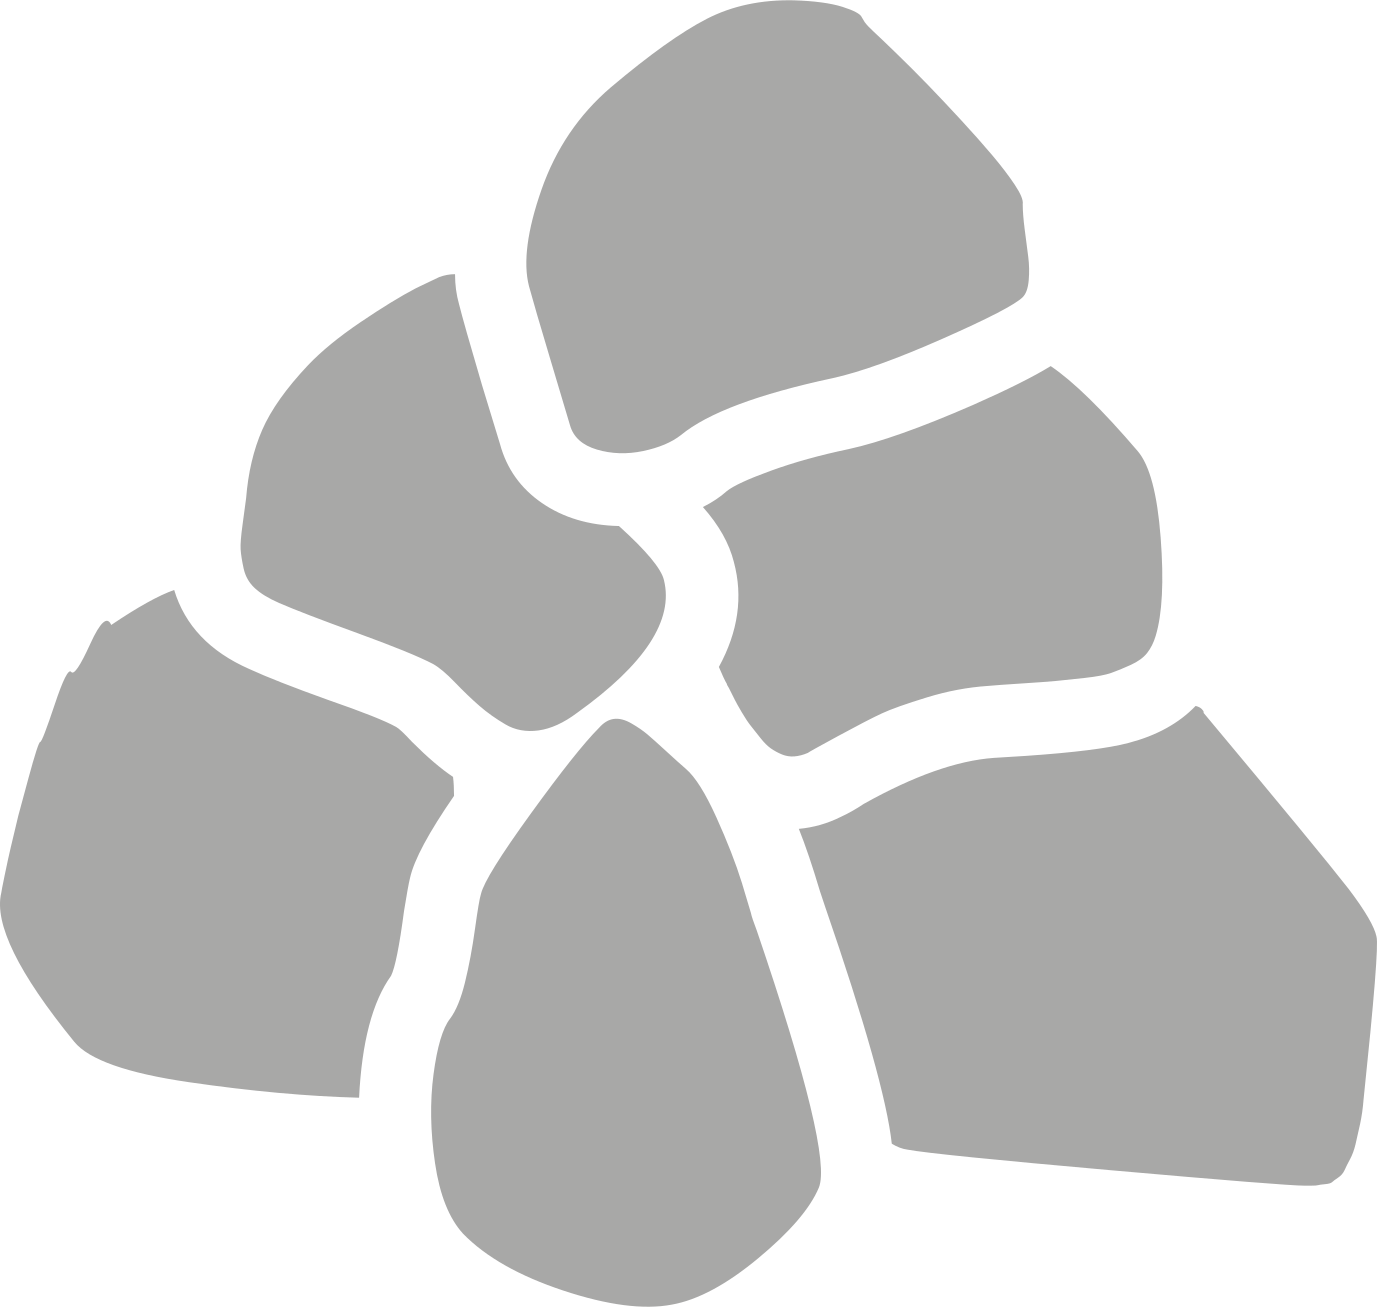
\includegraphics[scale=0.2]{\images/building_materials.png}
  \footnotesize\textcolor{darkcandyapplered}{\textit{\textbf{Building Materials}}}
  \columnbreak
  \vspace*{\fill}
  
\includegraphics[scale=0.2]{\images/valuables.png}
  \footnotesize\textcolor{darkcandyapplered}{\textit{\textbf{Valuables}}}
\end{multicols}
Players start each Scenario with the number of Resources indicated in that Scenario’s set up.
Resources can also be \hyperlink{Trading}{traded}.
There's no limit to the amount of Resources you can have.

\vspace*{\fill}

\columnbreak

\shadowimage[width=0.5\textwidth]{\images/resource_board.png}
\smallskip
\centering\footnotesize\textcolor{darkcandyapplered}{\textbf{\textit{Resource production tracker}}}
\bigskip

Possible Resource Die \includesvg[height=10px]{\svgs/resource_die.svg} results:
\medskip
\begin{itemize}
  \setlength\itemsep{8pt}
  \item \includesvg[height=15px]{\svgs/2BuildMat.svg} - 2 x Building Materials
  \item \includesvg[height=15px]{\svgs/4BuildMat.svg} - 4 x Building Materials
  \item \includesvg[height=15px]{\svgs/1valuables.svg} - 1 x Valuables
  \item \includesvg[height=15px]{\svgs/2valuables.svg} - 2 x Valuables
  \item \includesvg[height=15px]{\svgs/3gold.svg} 3 x Gold
  \item \includesvg[height=15px]{\svgs/6gold.svg} 6 x Gold
\end{itemize}

\end{multicols}

\vspace*{\fill}

\begin{figure*}[!hb]
  \centering
  \includegraphics[scale=0.095]{\art/griffin.jpg}
\end{figure*}
